\title{[Lab4] English Spelling Correction}
\author{0616014 楊政道}
\maketitle
\thispagestyle{fancy}
\section{Introduction}
\subsection{Lab Objective}
\paragraph{}
In this assignment, I will use long short-term memory recurrent neural networks to construct a sequence to sequence structure. In this structure, there are some parts in this structure including word embedding, encoder and decoder. Finally, I will use BLEU-4 score to measure the performance to the network output.
\subsection{Dataset}
\paragraph{}
There are many word pairs like (owrk, work) or (thign, thing). The first of the pair is the input word which is with some wrong and the second of the pair is the correct word we need to predict.
\subsection{Project Structure}
\dirtree{%
.1 DLP\_LAB4\_0616014\_楊政道.zip.
.2 dataset/.
.3 dataloader.py.
.2 model/.
.3 Encoder.py.
.3 Decoder.py.
.3 Seq2Seq.py.
.2 weight/.
.3 record.json.
.2 train.py.
.2 evaluate.py.
}
\subsubsection{data/dataloader.py}
\paragraph{}
To generate the dataloader for our training and testing data and it contains encode and decode function to convert the words between string and tensor.
\subsubsection{model/Encoder.py}
\paragraph{}
To define the structure of the encoder rnn.
\subsubsection{model/Decoder.py}
\paragraph{}
To define the structure of the decoder rnn.
\subsubsection{model/Seq2Seq.py}
\paragraph{}
To Combine encoder and decoder into one model and implement the train and predict function.
\subsubsection{weight/record.json}
\paragraph{}
To mentain the maximum test accuracy. If we have higher test accuracy, we will replace the weight and update the record file. The model parameters will be stored in weight directory.
\subsubsection{train.py}
\paragraph{}
To define the trainer function and train networks.
\subsubsection{evaluate.py}
\paragraph{}
It will load the network parameters we have stored and evaluate the network.
\section{Derivation of BPTT}
\paragraph{}
Assume that we have a sequence of data.
$$x^1, x^2, \dots, x^\tau$$
\paragraph{}
hidden units $h^t$ are
\begin{equation}
\begin{aligned}
h^t &= f_\theta(h^{t-1}, x^t)\\ &= f_\theta(f_\theta(h^{t-2}, x^{t-1}), x^t) \\ 
&=g^t(h^0, x^1, x^2, \dots, x^\tau)
\end{aligned}
\end{equation}
\subsection{Back-Propagation Through Time(BPTT)}
\paragraph{}
$$\nabla_WL = \sum_t{\sum_i{(\frac{\partial L}{\partial h_i^{t}})(\nabla_Wh_i^t)}}$$
\paragraph{}
Therefore, we need to compute $\nabla_{h^t}L$
\begin{equation}
\begin{aligned}
\nabla_{h^t}L &= (\frac{\partial h^{t+1}}{\partial h^{t}})^T(\nabla_{h^{t+1}}L) + (\frac{\partial o^{t}}{\partial h^t})^T(\nabla_{o^t}L) \\ &= W^TH^{t+1}(\nabla_{h^{t+1}}L)+V^T(\nabla_{o^t}L)
\end{aligned}
\end{equation}
\paragraph{}
where 
$$H^{t+1} = (\frac{\partial h^{t+1}}{\partial a^{t+1}})^T$$
$$\nabla_{o^t}L = \hat{y}^t - y^t$$
$$\nabla_{h^{\tau}}L = V^T(\nabla_{o^\tau}L)=V^T(\hat{y}^\tau - y^\tau)$$

\section{Implementation details}
\subsection{DataLoader}
\paragraph{}
In the dataloader, we need to implement a structure called dictionary, which it can help us to encode and decode between string and tensor.
\begin{lstlisting}[language=Python]
class Dictionary:

    def __init__(self, words):
        self.char2idx = {'SOS': 0, 'EOS': 1, 'UNK': 2}
        self.idx2char = {0: '', 1: '', 2: '?'}

        self.__analysis(words)

    def __analysis(self, words):
        for word in words:
            self.__analysis_word(word)

    def __analysis_word(self, word):
        for char in word:
            if char in self.char2idx:
                continue
            idx = len(self.char2idx)
            self.char2idx[char] = idx
            self.idx2char[idx] = char
        
    def encode(self, w):
        return torch.tensor(
              [ self.char2idx[c] if c in self.char2idx else 2 for c in w ]
            + [ 1 ],
        device=device).view(-1, 1)

    def decode(self, t):
        return ''.join([self.idx2char[v.item()] for v in t.view(-1)])

class DataLoader:

    def __init__(self, path):
        self.train_data = self.__load(path + "train.json", True)
        self.test_data  = self.__load(path + "test.json", False)
        self.dict = Dictionary(sum([ [ p[0], p[1] ] for p in self.train_data], []))

    def __load(self, path, base):
        with open(path, 'r') as f:
            return [ 
                (input, item['target']) for item in json.load(f) 
                for input in item['input'] + [item['target']] * base
            ]

    def encode(self, w):
        return self.dict.encode(w)

    def decode(self, t):
        return self.dict.decode(t)
\end{lstlisting}
\subsection{Encoder}
\paragraph{}
Encoder RNN contains a embedding function and a lstm. Embedding function can convert a scale into a vector and adjust the value during training stage.
\begin{lstlisting}[language=Python]
class EncoderRNN(nn.Module):

    def __init__(self, input_size, hidden_size):
        super(EncoderRNN, self).__init__()
        self.hidden_size = hidden_size
        self.embedding = nn.Embedding(input_size, hidden_size)
        self.lstm = nn.LSTM(hidden_size, hidden_size)

    def forward(self, input, hidden):
        embedded = self.embedding(input).view(input.size(0), 1, -1)
        output, hidden = self.lstm(embedded, hidden)
        return output, hidden

    def initHidden(self):
        return (
            torch.zeros(1, 1, self.hidden_size, device=device),
            torch.zeros(1, 1, self.hidden_size, device=device)
        )

    def name(self):
        return f'EncoderRNN-{self.hidden_size}'
\end{lstlisting}
\subsection{Decoder}
\paragraph{}
The decoder is similar to encoder, the only difference is the output of the decoder will go througe a fully-connected layer as a classifier.
\begin{lstlisting}[language=Python]
class DecoderRNN(nn.Module):

    def __init__(self, hidden_size, output_size):
        super(DecoderRNN, self).__init__()
        self.hidden_size = hidden_size
        self.embedding = nn.Embedding(output_size, hidden_size)
        self.lstm = nn.LSTM(hidden_size, hidden_size)
        self.out = nn.Linear(hidden_size, output_size)

    def forward(self, input, hidden):
        output = self.embedding(input).view(1, 1, -1)
        output = F.relu(output)
        output, hidden = self.lstm(output, hidden)
        output = self.out(output[0])
        return output, hidden

    def name(self):
        return f'DecoderRNN-{self.hidden_size}'
\end{lstlisting}
\subsection{Seq2Seq}
\paragraph{}
In the training stage, the sequence to sequence is to combine the encoder and decoder model. First, we will input the data stream into the encoder rnn and get a hidden value. Then, we will use a SOS\_token to wake up the decoder and the decoder will predict the output one by one according to the hidden state we are given. If the decoder outputs EOS\_token, it means that the decoder finishes the prediction and we will get the output tensor. Finally, we can compare this two tensor, calculate the gradient and update the weight of our networks.
\begin{lstlisting}[language=Python]
class Seq2Seq(nn.Module):

    def __init__(self, encoder, decoder):
        super(Seq2Seq, self).__init__()
        self.encoder = encoder
        self.decoder = decoder

    def forward(self, input, target, use_teacher_forcing):
        output, hidden = self.encoder(input, self.encoder.initHidden())
        input = torch.tensor([[0]], device=device)
        ret = []
        for i in range(MAX_LENGTH):
            output, hidden = self.decoder(input, hidden)
            if use_teacher_forcing:
                if i == target.size(0):
                    break
                ret.append(output)
                input = target[i]
            else:
                ret.append(output)
                topv, topi = output.topk(1)
                input = topi.squeeze().detach()
                if input.item() == 1:
                    break
        return torch.stack(ret)

    def name(self):
        return self.encoder.name() + '-' + self.decoder.name()
\end{lstlisting}
\paragraph{}
In the testing stage, we cannot use any information from the ground truth.
\begin{lstlisting}[language=Python]
class Seq2Seq(nn.Module):

    def predict(self, word, dataloader):
        word_tensor = dataloader.encode(word)
        output_tensor = self.forward(word_tensor, None, False).argmax(dim=2).view(-1, 1)
        output = dataloader.decode(output_tensor)
        return output

    def test(self, dataloader, display=False):
        total_bleu = 0
        for p in dataloader.test_data:
            output = self.predict(p[0], dataloader)
            total_bleu += compute_bleu(output, p[1])
            if not display or output == p[1]:
                continue
            print ('<', p[0])
            print ('=', p[1])
            print ('>', output)
        return total_bleu * 100 / len(dataloader.test_data)
\end{lstlisting}
\paragraph{}
When we want to predict, we call \texttt{self.forward(word\_tensor, None, False)} to not pass the target information into function and disable teacher forcing to make the decoder output from its previous output. Therefore, it can show that I don't use any ground truth information when prediction.
\section{Result}
\subsection{Loss plot}
\begin{figure}[!ht]
    \begin{center} 
        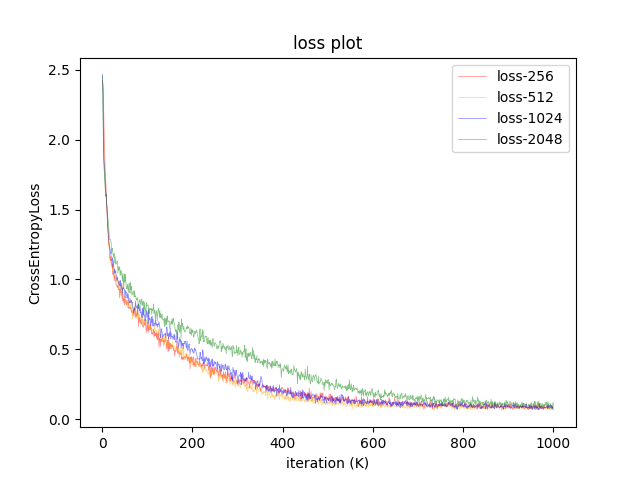
\includegraphics[width=8cm]{loss.png}
        \caption{Loss plot}
    \end{center} 
\end{figure}
\subsection{BLEU-4 score plot}
\begin{figure}[!ht]
    \begin{center} 
        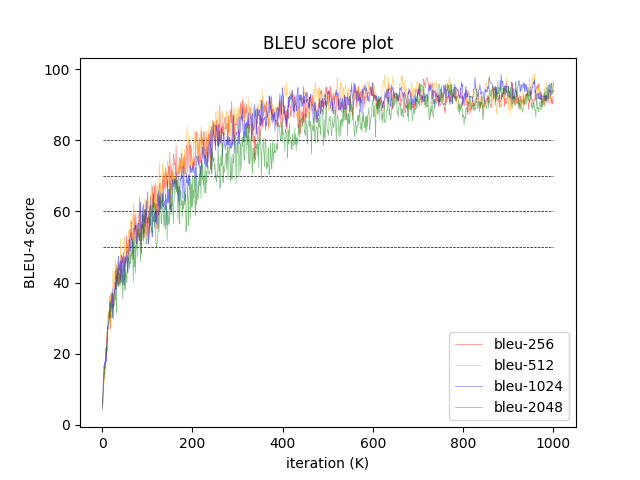
\includegraphics[width=8cm]{bleu.png}
        \caption{BLEU plot}
    \end{center} 
\end{figure}
\subsubsection{Test BLEU score}
\begin{center}
\begin{tabular}{ |c|c|  }
\hline
Model(Seq2Seq-\{hidden\_size\}) & Max Test BLEU\\
\hline
Seq2Seq-256 & 98.20\\
Seq2Seq-512 & 98.50\\
Seq2Seq-1024 & 98.50\\
Seq2Seq-2048 & 96.70\\
\hline
\end{tabular}
\end{center}
\subsection{Discussion}
\paragraph{}
We can find that the performance of the lstm recurrent neural network on the english correction task is good. The BLEU score of the test data can reach up to 98\%.
\paragraph{}
I find that there are many training pair which are two correct words in the same pair like (facilities, philosophy). Maybe the better method about the english spelling correction need to refer the contents before and after the target word.
\paragraph{}
Another method we can improve this sequence to sequence model is the attention mechanism. We can refer the data from encoder not only the hidden state but the output of the encoder. And use some weighted functions to emphasize the different part of the word to find the most important part. For example, if we want to correct the word \texttt{watchs}, the attention from the decoder may focus on the \texttt{ch} part and correct the word into \texttt{watches}. 
